% \documentclass[a4paper,10pt]{article}
\documentclass[review]{siamart}
\usepackage{url}
\usepackage{amssymb}
\usepackage{amsmath}
\usepackage{bm}
\usepackage{stmaryrd}
\usepackage{array}
\usepackage{multirow}
\usepackage{empheq}
\usepackage{enumitem}
	\setlist{nosep} % or \setlist{noitemsep} to leave space around whole list
\usepackage{color}
% \usepackage{showlabels}
\usepackage{adjustbox}
\usepackage{hyperref}
\definecolor{darkgreen}{rgb}{0.0, 0.5, 0}
\usepackage[numbers,sort]{natbib}
\usepackage{cleveref}

\newsiamremark{remark}{Remark}


% \newtheorem{lemma}{Lemma}
% \newtheorem{definition}{Definition}
% \newtheorem{theorem}{Theorem}
% \newtheorem{corollary}{Corollary}

\newcommand{\tcb}{\textcolor{blue}}
\newcommand{\tcp}{\textcolor{purple}}
\newcommand{\todo}[1]{\textcolor{red}{[TODO\@: #1]}}

\newcommand{\mdet}{\operatorname{det}}
\newcommand{\madj}{\operatorname{adj}}

% ------------------------------------------------------------------------------------ %
% ------------------------------------------------------------------------------------ %

\newcommand{\TheTitle}{Fast solution of fully implict Runge-Kutta\\systems in numerical PDEs}
\newcommand{\TheAuthors}{B.S. Southworth }
\headers{IRK!}{\TheAuthors}
\title{{\TheTitle}\thanks{This research was conducted ...
  }}

\author{%
  Ben~S.~Southworth
  \thanks{Department of Applied Mathematics,
          University of Colorado at Boulder
          (\email{ben.s.southworth@gmail.com}).}
}

\ifpdf%
\hypersetup{%
  pdftitle={\TheTitle},
  pdfauthor={\TheAuthors}
}
\fi

% ------------------------------------------------------------------------------------ %
% ------------------------------------------------------------------------------------ %

\begin{document}
\maketitle
\allowdisplaybreaks

\begin{abstract}

\end{abstract}


% ------------------------------------------------------------------------------------- %
% ------------------------------------------------------------------------------------- %
% ------------------------------------------------------------------------------------- %
\section{Introduction}

% ------------------------------------------------------------------------------------- %
% ------------------------------------------------------------------------------------- %
\subsection{Fully implicit Runge-Kutta}

Consider the method-of-lines approach to the numerical solution of partial differential
equations (PDEs), where we discretize in space and arrive at a system of ODEs in time,
%
\begin{align}\label{eq:problem}
	M\mathbf{u}'(t) =  \mathcal{N}(\mathbf{u},t) \quad\text{in }(0,T], \quad \mathbf{u}(0) = \mathbf{u}_0,
\end{align}
%
where $M$ is a mass matrix and $\mathcal{N}\in\mathbb{R}^{N\times N}$ is a discrete, time-dependent, nonlinear operator depending on $t$ and $\mathbf{u}$ (including potential
forcing terms). Then, consider time propagation using an $s$-stage Runge-Kutta scheme,
characterized by the Butcher tableaux 
%
\begin{align*}
	\renewcommand\arraystretch{1.2}
	\begin{array}
	{c|c}
	\mathbf{c}_0 & A_0\\
	\hline
	& \mathbf{b}_0^T
	\end{array},
\end{align*}
%
with Runge-Kutta matrix $A_0 = (a_{ij})$, weight vector $\mathbf{b}_0^T = (b_1, \ldots, b_s)^T$,
and quadrature nodes $\mathbf{c}_0 = (c_0, \ldots, c_s)$.

Runge-Kutta methods update the solution using a sum over stage vectors,
%
\begin{align*}
\mathbf{u}_{n+1} & = \mathbf{u}_n + \delta t \sum_{i=1}^s b_i\mathbf{k}_i, \\
M\mathbf{k}_i & = \mathcal{N}\left(\mathbf{u}_n + \delta t\sum_{j=1}^s a_{ij}\mathbf{k}_j, t_n+\delta tc_i\right).
\end{align*}
%
For nonlinear PDEs, $\mathcal{N}$ is linearized using, for example, a Newton or a Picard
linearization of the underlying PDE. Let us denote this linearization ${\mathcal{L}}\in\mathbb{R}^{N\times N}$
(or, in the case of a linear PDE, let $\mathcal{L} := \mathcal{N}$).
Expanding, solving for the stages $\mathbf{k}$ as each step in a nonlinear iteration, or
as the update to $\mathbf{u}$ for a linear PDE, can then be expressed as a block linear system,
%
\begin{align}\label{eq:k0}
\left( \begin{bmatrix} M  & & \mathbf{0} \\ & \ddots \\ \mathbf{0} & & M\end{bmatrix}
	- \delta t \begin{bmatrix} a_{11}\mathcal{L}_1 & ... & a_{1s}\mathcal{L}_1 \\
	\vdots & \ddots & \vdots \\ a_{s1}\mathcal{L}_s & ... & a_{ss} \mathcal{L}_s \end{bmatrix} \right)
	\begin{bmatrix} \mathbf{k}_1 \\ \vdots \\ \mathbf{k}_s \end{bmatrix} 
& = \begin{bmatrix} \mathbf{f}_1 \\ \vdots \\ \mathbf{f}_s \end{bmatrix}.
\end{align}
%

The difficulty in fully implicit Runge-Kutta methods (which we will denote IRK) lies in
solving the $Ns\times Ns$ block linear system in \eqref{eq:k0}. This paper focuses on the
parallel simulation of numerical PDEs, where $N$ is typically very large, on the order of
millions or billions, and $\mathcal{L}$ is highly ill-conditioned. In such cases, direct
solution techniques to solve \eqref{eq:k0} are not a viable option, and fast, parallel 
iterative methods must be used. However, IRK methods are rarely employed in practice due
to the difficulties of solving \eqref{eq:k0}. Even for relatively simple
parabolic PDEs where $\mathcal{L}$ is symmetric positive definite, \eqref{eq:k0}
instead yields a large nonsymmetric system with significant block coupling. For
nonsymmetric systems $\mathcal{L}$ that already have variable coupling, fast iterative
methods are even less likely to yield acceptable performance in solving \eqref{eq:k0}.

\todo{Add citations}
Although difficult to solve, there are a number of desirable properties of IRK schemes,
particularly in terms of accuracy and stabillity (\todo{why stability?}).
In practice, people typically use
diagonally implicit Runge-Kutta (DIRK) methods, where $A_0$ is lower triangular, or
singly implicit Runge Kutta (SIRK) methods, where $A_0$ has exactly one positive real
eigenvalue. For such schemes, the solution of \eqref{eq:k0} only requires $s$ linear
solves along the lines of $M - \delta ta_{ii}\mathcal{L}_i$. Unfortunately, SIRK and DIRK
schemes suffer from stage-order one (stage-order two with one explicit stage), and for
stiff nonlinear PDEs, the observed global order of accuracy in practice can be limited to
$\approx \min\{ p, q+1\}$, for integration order $p$ and stage-order $q$. Thus, even
a 6th-order DIRK method may only yield 2nd-order accuracy. For stiff problems, IRK
methods can achieve high stage order (although not as high as the formal accuracy of
the method), and thus result in high-order global accuracy. Furthermore, for less stiff
problems, IRK methods can yield accuracy as high as order $2s$ for an $s$ stage method,
compared with a maximum of $s$ or $s+1$ for SDIRK methods with reasonable stability
properties \cite[Section IV.6]{hairer96}.

One simplification for using IRK methods in practice is to assume $\mathcal{L}_i =
\mathcal{L}_j$ for all $i,j$, that is, $\mathcal{L}$ has no dependence on time. Such
an assumption is natural for linear problems with no time-dependence in the spatial
differential components, or when applying a simplified Newton method to nonlinear
problems, where the Jacobian is only evaluated at one time-point per outer RK time
step. Either case yields a simplified form of \eqref{eq:k0} that can be expressed in
Kronecker product form,
%
\begin{align}\label{eq:kron1}
(I\otimes M - \delta t A_0\otimes \mathcal{L})\mathbf{k} & = \mathbf{f},
\end{align}
%
where $\mathcal{L}$ is a fixed real-valued spatial operator or Jacobian.
Here, we revive some of the older Runge-Kutta work in the light of a changing
computational landscape, developing a fast, parallel preconditioning technique for
\eqref{eq:kron1}. The new method effectively requires $s$ real-valued linear solves
of matrices along the lines of $\eta M - \delta t\mathcal{L}$, for some $\eta > 1$,
and is easily implemented using existing preconditioners and parallel software libraries.
In contrast to other works that have considered the preconditioning of \eqref{eq:kron1}
via some form of splitting, the proposed algorithm here (i) is amenable to short-term
Krylov recursion (conjugate gradient/MINRES) if $M - \mathcal{L}$ is, and (ii) only
requires operating on systems of size $N$, an $s\times$ reduction in memory-usage of
Krylov solvers compared with directly preconditioning the larger system. In addition,
some of the results generalize to the weaker scenario of commuting spatial operators,
$\mathcal{L}_i\mathcal{L}_j = \mathcal{L}_j\mathcal{L}_i$, which provides a first step
towards the fast solution of time-dependent IRK.

\todo{outline sections}

% ------------------------------------------------------------------------------------- %
% ------------------------------------------------------------------------------------- %
\subsection{Previous work}\label{sec:intro:prev}

% To avoid complex arithmetic, one can pose each complex
% system as a real $2\times 2$ block system,
% Because eigenvalues come in conjugate pairs, we will
% instead consider inverting conjugate pairs $(\overline{\lambda_i}I - \mathcal{L})^{-1}
% = \overline{(\lambda_iI - \mathcal{L})^{-1}}$, and thus the same solver/preconditioner
% could be used for conjugate pairs of eigenvalues \todo{cite}. However, this does not
% solve the underlying problem of constructing complex solvers/preconditioners in
% practice. 

Many papers have considered the solution of \eqref{eq:kron1} over the years. In 1976,
Butcher \cite{butcher76} used the Jordan normal form, $A_0 = U_0L_0U_0^{-1}$, where
$L_0$ is lower triangular with eigenvalues of $A_0$ on the diagonal, to transform
\eqref{eq:kron1} to the problem
$(I\otimes M - \delta t L_0\otimes \mathcal{L})(U_0^{-1}\otimes I)\mathbf{k} =
(U_0\otimes I)^{-1}\mathbf{f}$, where the inner operator is now block lower triangular.
Such a transformation reduces the solution of an $Ns\times Ns$ system to $s$ linear
systems of size $N\times N$ in a block forward solve. The downside is that
IRK schemes with greater accuracy and stability than DIRK schemes have at most one real
eigenvalue \cite{hairer96,butcher2016numerical}.
Thus, for IRK methods such as Gauss or Radau integration, the original real-valued
system is transformed into a set of smaller but primarily complex systems. There are various
ways to handle the complex systems,
but for numerial PDEs, the overhead in computational cost and implementation is typically
too high to make the transformation a practical approach.  

Published shortly after (and independently from) Butcher, Bickart proposed a similar
way to invert \eqref{eq:kron1} \cite{bickart77}. If we define $Q_s(x)$ as
the characteristic polynomial of $A_0$, then the inverse of \eqref{eq:kron1} can be computed
via a specific set of matrix-vector multiplications in addition to the action of
$Q_s(\mathcal{L})^{-1}$.
In principle this is similar to Butcher's result, as one can invert
$Q_s(\mathcal{L})$ by inverting 
each term in the factored polynomial, $(\mu_1 I-\mathcal{L})^{-1}$,
$(\mu_2 I-\mathcal{L})^{-1}$, ..., for eigenvalues $\{\mu_i\}_{i=1}^s$ of $A_0$.
Although Bickart's paper received less attention than Butcher's over time (currently $2.5\times$
less citations), the polynomial form provides a more natural way to handle complex eigenvalues,
particularly for numerical PDEs in the modern high-performance computing landscape,
where direct LU inverses are rare and most linear systems are solved via preconditioning
and/or Krylov methods. We present a similar result in \Cref{lem:inv} and use this to
develop an effective preconditioning in \Cref{sec:solve:prec}.

Because significant research has been done on IRK methods, it is worth briefly
reviewing some of the literature to put this work in context. In the field of time
integration, SIRK and DIRK methods overcome the difficulty of solving IRK methods
\cite{alexander1977diagonally,norsett1976runge}.
In \cite{orel91}, it is shown that in considering RK methods with all real eigenvalues
(wherein the Butcher transformation \cite{butcher76} remains real-valued), the best
approximation to exponential is obtained by having all eigenvalues equal (SIRK
methods \cite{norsett1976runge}).
Although SIRK methods offer some advantages over DIRK methods, they generally lack
the favorable stability and accuracy of IRK methods \cite{orel91}. ESIRK methods
use one explicit stage and can offer stage-order two \cite{butcher00} (one higher
than standard SIRK methods), which provide an improved practical option, but still
lack the robustness of fully implicit methods.




% Simplified newton scheme uses fixed Jacobian for all stages
% Single step Newton (Cooper (83/90), Gonzales-Pinto (95/97)
% ---------------- ODEs and LU ---------------- %
% Butcher (76), Bickart (77)
% \begin{itemize}
% 	\item Uses tensor product structure, gets Jordan normal form of Butcher matrix A. Reformulates
% 	problem as block subdiagonal, with diagonal blocks $I - h\lambda J$, for Jacobian $J$, time step $h$,
% 	and eigenvalue $\lambda$ of $A$ (are we sure not $A^{-1}$??).
% 	\item Must solve for complex eigenvalues. This is not desirable. 
% 	\item Bickart uses polynomial form, closer to what I look at. Originally based on Tensor product
% 	result from Jameson (68)
% \end{itemize}

% Varah (79):
% \begin{itemize}
% 	\item Much better description of Butcher's method. Transforms coordinate system of Jacobian tensor.
% 	Still relies on this tensor structure to do said transformation. 
% 	\item Transforms Jacobian to Hessenberg form to avoid repeated action computing LU of a shifted 
% 	Jacobian.
% \end{itemize}

% Burrage (82):
% \begin{itemize}
% 	\item Look at stability of DIRK and SIRK methods, which have one eigenvalue and are more amenable
% 	to development by Butcher. 
% \end{itemize}

% Orel (91):
% \begin{itemize}
% 	\item Looks at RK methods w/ real eigenvalues. Turns out best approximation to exponential is
% 	obtained by having all eigenvalues equal (SIRK/SDIRK methods). SIRK methods offer some advantages over SDIRK methods, but lack the favorable stabillity an accuracy of IRK methods. 
% \end{itemize}

% Cooper:
% \begin{itemize}
% 	\item (83,90,93): develops single Newton scheme using SOR or various matrix splittings,
% 	applied to ODEs. This is a single-step
% 	Newton method, where the actual Jacobian solve is replaced with an SOR iteration. Here, Butcher
% 	matrix A is replaced with an approximate matrix with one positive real eigenvalue. 
% \end{itemize}

% Pinto:
% \begin{itemize}
% 	\item (95) Mostly ODEs, do consider 1d-space-1d-time burgers on a very small grid. 
% 	\item (96) additional iteration of single Newton, makes it quasi-Newton like. 
% 	\item (01) Analysis of single Newton (SOR) w/ simplified Newton for higer order. 
% \end{itemize}


% Butcher (2000):
% \begin{itemize}
% 	\item Develops ESDIRK schemes w/ higher stage order and stiff accuracy than traditional
% 	SIRK/DIRK schemes. Based on using iniital explicit stage, moves RK abscissae.
% \end{itemize}


% Brugano (2014) and Antonana (2018)
% \begin{itemize}
% 	\item New splitting and IRK techniques for Hamiltonian problems where conservation is
% 	important. Used for ODEs. 
% \end{itemize}


% % ---------------- PDEs ---------------- %

% \begin{itemize}
% 	\item One obvious drawback -- even if spatial operator/Jacobian is SPD, IRK system is
% 	nonsymmetric.
% \end{itemize}

% Jay
% \begin{itemize}
% 	\item 1999: develops a preconditioning technique based on W-transformation. W-transformation
% 	yields a real-valued block-tridiagonal matrix. This can be solved using LU, but the inverses
% 	have a recursive nature (like Schur complements). They precondition w/ an approximate LU,
% 	where each formal inverse in LU is approximated, $H_i = I +
% 	\zeta_{i-1}^2\delta t^2 JH_{i-1}^{-1}J$, for Jacobian $J$ and matrix $H$ that must be
% 	inverted in LU, with $\hat{H}_i = I - \gamma_i\delta tJ$, for a certain \gamma_i$. 

% 	\item 2000: Analyzes simplified Newton to approximate time-dependent Jacobian with
% 	Kronecker product form. 
% \end{itemize}

% Houwen 
% \begin{itemize}
% \item TRIANGULARLY(1997): Uses crout factorization to pick lower triangular preconditioner.
% \item Paralell(97): 
% \end{itemize}

% Hoffman 
% \begin{itemize}
% \item (97): Also uses triangular preocnditioner on the nonlinear level.
% \end{itemize}


% Van Lent (2004)
% \begin{itemize}
% 	\item Multigrid for IRK?
% \end{itemize}

% Staff \& Mardal (2006)
% \begin{itemize}
% 	\item One of first paper to consider preconditioning the fully implicit RK system.
% 	Use block Jacobi and block lower triangular preconditioners for the diffusion equation.
% 	Use multigrid V-cycles and full Newton time-dependent Jacobian. Upper triangular is
% 	bad compared to block Jacobi and lower triangular (this has appeared elsewhere in
% 	literature -- $A_0$ is dominant in lower triangular part -- Crout factorization
% 	in I think Messina or Van der Houwen; comes up again in Brugano (2015)).
% \end{itemize}
% Mardal (2007)
% \begin{itemize}
% 	\item Analyze block-diagonal preconditioners in a Sobolev setting, demonstrate
% 	conditioning of the preconditioned operator to be optimal in the independent of
% 	$h$ sense. Use multigrid w/ diffusion as example. 
% \end{itemize}
% Nilssen (2011)
% \begin{itemize}
% 	\item Analogous to above, Sobolev analysis for block-diagonal preconditioning
% 	applied to the bidomain equations.
% \end{itemize}

% Xie (2011)
% \begin{itemize}
% 	\item Proposes a modified simplified Newton for the time-dependent cast, where the Jacobian is
% 	formed based on a least squares approximation to the true RK coefficients, evaluating all entries
% 	at a single time point. In example problems, modified Jacobian typically converged faster
% 	than simplified (evaluated at previous time step), up to 2x less iterations/time. 
% \end{itemize}

% Hao Chen:
% \begin{itemize}
% 	\item (2014) Develops a splitting iterative method to precondition IRK matrices, similar to ADI schemes.
% 	Proves that for definite spatial operators and Butcher matrices (that is, eignvalues have positive
% 	or negative real parts), $\rho(T) < 1$, where $T$ is the fixed-point iteration matrix. Look at 
% 	diffusion equation with IRK and BVMs.
% 	\item (2016) Analogous to above, extended to wave equation.
% \end{itemize}

% Pazner
% \begin{itemize}
% 	\item
% \end{itemize}

% \begin{itemize}
% 	\item if the underlying IRK methods are A-stable, irreducible, and have invertible coefficientmatrixA, such as Gauss, RadauIIA, and LobattoIIIC (cf., e.g., [Hairer]), then the real partsof the eigenvalues ofAare positive,
% 	\item One benefit of this method is ability to use PCG or GMRES on smaller system, not full system. 
% \end{itemize}


% ------------------------------------------------------------------------------------- %
% ------------------------------------------------------------------------------------- %
% ------------------------------------------------------------------------------------- %
\section{Fast parallel solvers for IRK}\label{sec:solve}

The fully implicit RK stage system in \eqref{eq:k0} can be reformulated by pulling out 
an $A_0^{-1}$ as \cite{pazner17}
%
\begin{align}\label{eq:keq}
\left( A_0^{-1}\otimes M - \delta t \begin{bmatrix} \mathcal{L}_1  & \\ & \ddots \\ && \mathcal{L}_s\end{bmatrix}\right)
	(A_0\otimes I)	\begin{bmatrix} \mathbf{k}_1 \\ \vdots \\ \mathbf{k}_s \end{bmatrix} 
& = \begin{bmatrix} \mathbf{f}_1 \\ \vdots \\ \mathbf{f}_s \end{bmatrix}.
\end{align}
%
For ease of notation, let us scale both sides of the system by a block-diagonal mass matrix 
and, excusing the slight abuse of notation, let
%
\begin{equation*}
\widehat{\mathcal{L}}_i := \delta t M^{-1}\mathcal{L}_i,
\end{equation*}
%
for $i=1,..,s$. Note the time step $\delta t$ for the given Runge-Kutta step is now included in $\widehat{\mathcal{L}}_i$. Now let $\alpha_{ij}$ denote the $ij$-element of $A_0^{-1}$ (assuming $A_0$ is
invertible). Then, solving \eqref{eq:k0} can be effectively reduced to inverting the operator
%
\begin{align}\nonumber
\mathcal{M}_s & := A_0^{-1}\otimes I - \begin{bmatrix} \widehat{\mathcal{L}}_1  & \\ & \ddots \\ && \widehat{\mathcal{L}}_s\end{bmatrix} \\
& = \begin{bmatrix} \alpha_{11}I - \widehat{\mathcal{L}}_1 & \alpha_{12}I & ... & \alpha_{1s}I \\
	\alpha_{21}I & \alpha_{22}I - \widehat{\mathcal{L}}_2 & & \alpha_{2s}I \\
	\ddots & & \ddots & \vdots \\ \alpha_{s1}I & ... & \alpha_{s(s-1)}I & \alpha_{ss}I - \widehat{\mathcal{L}}_s \end{bmatrix}.
	\label{eq:k1}
\end{align}
%

Note, there are a number of methods with one explicit stage preceded or followed by several
fully implicit and coupled stages. In such cases, $A_0$ is
not invertible, but the explicit stage can be eliminated from the system (by doing an explicit
time step). The remaining operator can then be reformulated as above, and the inverse that
must be applied takes the form of \eqref{eq:k1} but based on a principle submatrix of $A_0$.

% ------------------------------------------------------------------------------------- %
% ------------------------------------------------------------------------------------- %
\subsection{An inverse and update for commuting operators}\label{sec:solve:inv}

This section introduces a result similar to Bickart's \cite{bickart77},
but generalized to hold for commuting
operators. If $\widehat{\mathcal{L}}_i=\widehat{\mathcal{L}}_j$ for all $i,j$, we show that
the inverse of \eqref{eq:k1} can be expressed in terms of $P_s(\widehat{\mathcal{L}})^{-1}$,
where $P_s(\widehat{\mathcal{L}})$ is the characteristic polynomial of $A_0^{-1}$. Note, we
consider $\mathcal{M}_s$ as a matrix over the commutative ring of linear combinations of
$\{I, \mathcal{L}\}$, and the determinant and adjugate referred to in
\Cref{lem:inv} are defined over matrix-valued elements rather than scalars.

%
\begin{lemma}\label{lem:inv}
Let $\alpha_{ij}$ denote the $(i,j)$th entry of $A_0^{-1}$ and assume
$\{\widehat{\mathcal{L}}_i\}_{i=1}^s$ are commuting operators. Define $\mathcal{M}_s$
% \begin{align*}
% \mathcal{M}_s := \begin{bmatrix} \alpha_{11}I - \widehat{\mathcal{L}}_1 & \alpha_{12}I & ... & \alpha_{1s}I \\
% 	\alpha_{21}I & \alpha_{22}I - \widehat{\mathcal{L}}_2 & & \alpha_{2s}I \\
% 	\ddots & & \ddots & \vdots \\ \alpha_{s1}I & ... & \alpha_{s(s-1)}I & \alpha_{ss}I - \widehat{\mathcal{L}}_s \end{bmatrix},
% \end{align*}
as in \eqref{eq:k1}.
Let det$(\mathcal{M}_s)$ be the determinant of $\mathcal{M}_s$ (in this case a block-diagonal
matrix) and let adj$(\mathcal{M}_s)$ be the adjugate of $\mathcal{M}_s$. Then, $\mathcal{M}_s$
is invertible if and only if det$(\mathcal{M}_s)$ is invertible, and
\begin{align*}
\mathcal{M}_s^{-1} = \textnormal{det}(\mathcal{M}_s)^{-1}\textnormal{adj}(\mathcal{M}_s).
\end{align*}
%

Now, suppose $\widehat{\mathcal{L}}_i = \widehat{\mathcal{L}}_j$ for all $i,j$, and let $P_s(x)$ be the
characteristic polynomial of $A_0^{-1}$. Then,
\begin{align*}
\mathcal{M}_s^{-1} = \textnormal{diag}(P_s(\widehat{\mathcal{L}})^{-1})\textnormal{adj}(\mathcal{M}_s),
\end{align*}
where ``diag'' indicates a block diagonal matrix, with diagonal blocks given by $P_s(\widehat{\mathcal{L}})^{-1}$.
\end{lemma}
%
\begin{proof}
Notice in \eqref{eq:k1} that if $\widehat{\mathcal{L}}_i$ and $\widehat{\mathcal{L}}_j$ commute for all $i,j$,
then $\mathcal{M}_s$ is a matrix over the commutative ring of linear combinations
of $I$ and $\{\widehat{\mathcal{L}}_i\}$. Let adj$(\mathcal{M}_s)$ denote the matrix adjugate. A
classical result in matrix analysis then tells us that
%
\begin{align*} 
\textnormal{adj}(\mathcal{M}_s)\mathcal{M}_s = \mathcal{M}_s\textnormal{adj}(\mathcal{M}_s)
	= \textnormal{det}(\mathcal{M}_s)I.
\end{align*}
%
Moreover, $\mathcal{M}_s$ is invertible if and only if if the determinant of $\mathcal{M}_s$
is invertible, in which case $\mathcal{M}_s^{-1} := $ det$(\mathcal{M}_s)^{-1}$adj$(\mathcal{M}_s)$
\cite[Theorem 2.19 \& Corollary 2.21]{brown1993matrices}
For the case of time-independent operators ($\widehat{\mathcal{L}}_i=\widehat{\mathcal{L}}_j$), notice that
$\mathcal{M}_s$ takes the form $A_0^{-1} - \widehat{\mathcal{L}}I$ over the commutative ring defined
above. Analogous to a scalar matrix, the determinant of $A_0^{-1} - \widehat{\mathcal{L}}I$ is the
characteristic polynomial of $A_0^{-1}$ evaluated at $\widehat{\mathcal{L}}$.
\end{proof}
%

Returning to \eqref{eq:keq}, we can express the direct solution for the set of all
stage vectors ${\mathbf{k}} = [\mathbf{k}_1; ...; \mathbf{k}_s]$ as
%
\begin{align*}
\mathbf{k} &:= \textnormal{det}(\mathcal{M}_s)^{-1}
	(A_0^{-1}\otimes I)\textnormal{adj}(\mathcal{M}_s)\mathbf{f},
\end{align*}
%
where $\mathbf{f} = [\mathbf{f}_1; ...; \mathbf{f}_s]$ (note that
$A_0\otimes I$ commutes with $\textnormal{det}(\mathcal{M}_s)^{-1}$). Excusing the slight
abuse in notation, let $\textnormal{det}(\mathcal{M}_s)^{-1}$ now denote just the diagonal
block (rather than a block-diagonal matrix). The Runge-Kutta update is then given by
%
\begin{align}\nonumber
\mathbf{u}_{n+1} & = \mathbf{u}_n + \delta t\sum_{i=1}^s b_i{\mathbf{k}}_i \\
& = \mathbf{u}_n + \delta t\textnormal{det}(\mathcal{M}_s)^{-1}
	(\mathbf{b}_0^TA_0^{-1}\otimes I)\textnormal{adj}(\mathcal{M}_s)\mathbf{f}.\label{eq:update}
\end{align}
%

The adjugate simply consists of linear combinations of $I$ and $\widehat{\mathcal{L}}$, and an
analytical form can be derived for an arbitrary $s\times s$ matrix, where $s\sim\mathcal{O}(1)$.
Computing this operator analytically is easiest using a computer algebra program
such as Mathematica. Applying its action will consist of some set of vector summations
and matrix-vector multiplications. In particular, the diagonal elements of
$\textnormal{adj}(\mathcal{M}_s)$ are monic polynomials in $\widehat{\mathcal{L}}$ of degree
$s-1$ (or linear combinations of comparable degree if $\widehat{\mathcal{L}}_i\neq\widehat{\mathcal{L}}_j$)
and off-diagonal terms are polynomials in $\widehat{\mathcal{L}}$ of degree $s-2$. 

Returning to \eqref{eq:update}, we consider two cases. First, if a given Runge-Kutta
scheme is stiffly accurate (for example, RadauIIA methods),
then $\mathbf{b}_0^TA_0^{-1} = [0,...,0,1]$. This yields
the nice simplification that computing the update in \eqref{eq:update} only requires
applying the last row of $\textnormal{adj}(\mathcal{M}_s)$ to $\mathbf{f}$ (in a
dot-product sense) and applying $\textnormal{det}(\mathcal{M}_s)^{-1}$ to the result. From
the discussion above regarding the adjugate structure, applying the last row of
$\textnormal{adj}(\mathcal{M}_s)$ requires $(s-2)(s-1) + (s-1) = (s-1)^2$ matrix-vector
multiplications. Because this only happens once, followed by the linear solve(s),
these multiplications are typically of relatively marginal cost.

In the more general case of non stiffly accurate (for example, Gauss methods), one can
obtain an analytical form for
$(\mathbf{b}_0^TA_0^{-1}\otimes I)\textnormal{adj}(\mathcal{M}_s)$. Each element in
this matrix consists of polynomials in $\widehat{\mathcal{L}}$ of degree $s-1$ (although
typically not monic). Compared with stiffly accurate schemes, this now requires 
$(s-1)s$ matrix-vector multiplications, which is $s-1$ more than for stiffly
accurate schemes, but still typically of marginal overall computational cost. 

% ------------------------------------------------------------------------------------- %
% ------------------------------------------------------------------------------------- %
\subsection{Stability and the method of lines}\label{sec:solve:stab}

{\color{blue}
\begin{itemize}

\item A necessary condition for stable time-propagation is that eigenvalues of $\widehat{\mathcal{L}}$
lie in the region of stability for the given RK scheme. For virtually all implicit RK schemes,
this means that eigenvalues of $\widehat{\mathcal{L}}$ must have negative real part, or real part
$\gg 0$. It is rare for operators representing a differential discretization to be split
with a set of negative definite eigenvalues and a set of eigenvalues with real part $\gg 0$,
so for our purposes assume $\widehat{\mathcal{L}}$ has eigenvalues with negative real part.

\item Just eigenvalues is not strong enough for our analysis or stability. Need to look
into literature. Would be nice if it was related to numerical range/field of values, because
that is what our analysis is based on. Ideally, something along the lines of $\widehat{\mathcal{L}}$ 
has a non-positive field of values for stability? 
\end{itemize}
}


% ------------------------------------------------------------------------------------- %
% ------------------------------------------------------------------------------------- %
\subsection{Preconditioning by conjugate pairs}\label{sec:solve:prec}

Following the discussion and algorithm developed in \Cref{sec:solve:inv}, the key
outstanding point is inverting $\textnormal{det}(\mathcal{M}_s)^{-1}$. Moving forward, we
restrict our attention to the case $\widehat{\mathcal{L}}_i = \widehat{\mathcal{L}}_j$ for all $i,j$,
in which case $\textnormal{det}(\mathcal{M}_s)^{-1} = P_s(\widehat{\mathcal{L}})^{-1}$, where
$P_s(x)$ is the characteristic polynomial of $A_0^{-1}$ (see \Cref{lem:inv}).

In contrast to much of the original work on solving IRK systems, where LU factorizations
were the dominant cost and system sizes relatively small, explicitly forming and inverting
$P_s(\widehat{\mathcal{L}})$ for numerical PDEs is typically not a viable option in high-performance
simulation on modern computing architectures. Instead, by computing the eigenvalues
$\{\lambda_i\}$ of $A_0^{-1}$, we can express $P_s(\widehat{\mathcal{L}})$ in a factored form, 
%
\begin{align}\label{eq:fac}
P_s(\widehat{\mathcal{L}}) = \prod_{i=1}^s (\lambda_i I - \widehat{\mathcal{L}}),
\end{align}
%
and its inverse can then be computed by successive applications of $(\lambda_iI - \widehat{\mathcal{L}})^{-1}$,
for $i=1,...,s$. As discussed previously, eigenvalues of $A_0$ and $A_0^{-1}$ will often be
complex, making the inverse of individual factors $(\lambda_iI - \widehat{\mathcal{L}})^{-1}$ more
difficult and often impractical. 

Here, we propose combining pairs of conjugate eigenvalues into quadratic polynomials
that we must precondition, which take the form 
%
\begin{align}\label{eq:imag1}
\begin{split}
\mathcal{Q}_\eta :&= ((\eta + i\beta)I - \widehat{\mathcal{L}})((\eta - i\beta)I - \widehat{\mathcal{L}}) \\
& = (\eta^2+\beta^2)I - 2\eta \widehat{\mathcal{L}} + \widehat{\mathcal{L}}^2 
= (\eta I - \widehat{\mathcal{L}})^2 + \beta^2I. 
\end{split}
\end{align}
%
In practice, we typically do not want to directly form or precondition a quadratic
operator like \eqref{eq:imag1}, due to (i) the overhead cost of large parallel matrix
multiplication, and (ii) the fact that many fast parallel methods such as multigrid are not well-suited for solving a polynomial in $\widehat{\mathcal{L}}$. The point of \eqref{eq:imag1}
is that by considering conjugate pairs of eigenvalues, the resulting operator is real-valued.
Thus, consider preconditioning \eqref{eq:imag1} with the inverse of the real-valued quadratic
polynomial, $(\eta I - \widehat{\mathcal{L}})^2$, dropping the $+ \beta^2 I$ term. Expanding,
the preconditioned operator then takes the form
%
\begin{align}\nonumber
\mathcal{P}_\eta & := (\eta I - \widehat{\mathcal{L}})^{-2}\left[(\eta^2+\beta^2)I - 2\eta \widehat{\mathcal{L}} + \widehat{\mathcal{L}}^2\right] \\
&\hspace{5ex} = I + \beta^2(\eta I - \widehat{\mathcal{L}})^{-2}
= I + \frac{\beta^2}{\eta^2}\left(I - \tfrac{1}{\eta}\widehat{\mathcal{L}}\right)^{-2}.\label{eq:prec1}
\end{align}
%

It turns out, by reasonable assumptions on $\widehat{\mathcal{L}}$ that yield a stable
time-propagation scheme \todo{reference?}, the preconditioned operator in \eqref{eq:prec1}
is very well-conditioned.  \Cref{th:fov} analyzes the field-of-values of $\mathcal{P}_\eta$,
denoted $W(\mathcal{P}_\eta)$, as a measure of the preconditioning, and \Cref{cor:gmres} extends
this preconditioning to prove fast convergence of GMRES. 

%
\begin{remark}[Convergence independent of problem size]
It is worth pointing out the key
cancellation in \eqref{eq:prec1}, where the preconditioned operator has no terms directly
involving $\widehat{\mathcal{L}}$ or $\widehat{\mathcal{L}}^{-1}$ (why $(I -
\tfrac{1}{\eta}\widehat{\mathcal{L}})^{-2}$ is different will be clear in the proof
of \Cref{th:fov}). Because of this, the conditioning of $\mathcal{P}_\eta$ is effectively
independent of the conditioning of $\widehat{\mathcal{L}}$, which ensures convergence
that is independent of problem size. This is in contrast to most standard matrix-splitting
or block-preconditioning techniques, where the preconditioned operator has some dependence
on $\widehat{\mathcal{L}}$, which leads to convergence dependent on the conditioning of
$\widehat{\mathcal{L}}$ (and, thus indrectly, problem size).
\end{remark}
%

%
\begin{theorem}[Preconditioned field of values]\label{th:fov}
Assume that $\eta > 0$ and the symmetric part of $\widehat{\mathcal{L}}$ satisfies
$(\widehat{\mathcal{L}}+\widehat{\mathcal{L}}^T)/2 \leq 0$. Let $\mathcal{P}_\eta$ denote the preconditioned
operator, where $((\eta + i\beta)I - \widehat{\mathcal{L}})((\eta - i\beta)I - \widehat{\mathcal{L}})$ is
preconditioned with $(\eta I - \widehat{\mathcal{L}})^{-2}$. Then $W(\mathcal{P}_\eta)$ is bounded
by $\Omega$ as shown in \Cref{fig:bound}.
\begin{figure}[h!]
\centering
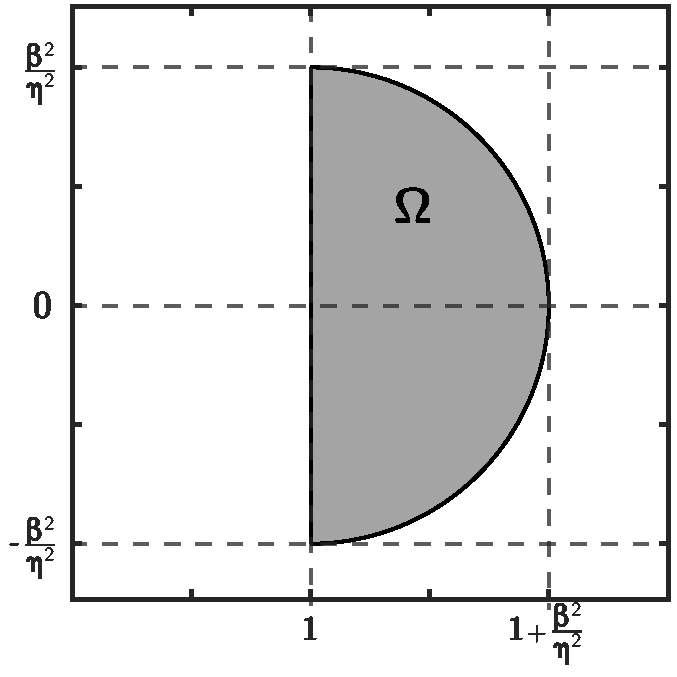
\includegraphics[width = 0.3\textwidth]{fov.pdf}
\caption{}
\label{fig:bound}
\end{figure}
\end{theorem}
\begin{proof}
Let $\sigma(B)$ denote the spectrum of operator $B$, $\sigma_{\textnormal{min}}(B)$
and $\sigma_{\textnormal{max}}(B)$ the minimum and maximum eigenvalues, and $\rho(B)$
the spectral radius. Also, define the symmetric/skew-symmetric splitting
$B = B_s + B_k$, where $B_s := (B+B^T)/2$ and $B_k := (B - B^T)/2$, and the numerical
radius as $r(B) = \sup \{ |\lambda| : \lambda \in W(B) \}$. Recall
the following properties of $W(B)$ \cite{gustafson1997numerical}:
%
\begin{enumerate}
	\item $W(B)\subset [\sigma_{\textnormal{min}}(B_s), \sigma_{\textnormal{max}}(B_s)] \times
	[-\rho(B_k)\mathrm{i}, \rho(B_k)\mathrm{i}]$.

	\item $\sigma(B) \subset W(B)$.

	% <Bv,v> + <v,Bv> > 0 ---> w = B^{-1}v ---> <w, B^{-1}w> + <B^{-1}w,w> > 0
	\item If $B$ is invertible and $B_s \leq 0$ in the symmetric negative semi-definite
	sense, then the symmetric part of $B^{-1}$ is also negative semi-definite.

	\item $r(B) \leq \|B\|_2$.

	\item $W(I + B) = 1 + W(B)$.
\end{enumerate}
%
Note that an exact inverse yields $\mathcal{P}_\eta = I$, with spectrum
and field-of-values given by $\sigma(\mathcal{P}_S) = W(\mathcal{P}_S) = \{1\}$.
Appealing to \eqref{eq:prec1} and the final property stated above, $W(\mathcal{P}_\eta)
= 1 + \tfrac{\beta^2}{\eta^2}W(E)$, for error term $E := (I - \tfrac{1}{\eta}\widehat{\mathcal{L}})^{-2}$
and real-valued constant $\beta^2/\eta^2 > 0$. Next we will bound $W(E)$ in the complex plane.

Assume that $\eta > 0$ and the symmetric part of $\widehat{\mathcal{L}}$ satisfies
$(\widehat{\mathcal{L}}+\widehat{\mathcal{L}}^T)/2 \leq 0$.
It follows that the real part of eigenvalues of $\widehat{\mathcal{L}}$ are non-positive and,
thus, $(I - \tfrac{1}{\eta}\widehat{\mathcal{L}})$ cannot have a zero eigenvalue and must be
invertible. Furthermore, it also follows that the symmetric part of
$(I - \tfrac{1}{\eta}\widehat{\mathcal{L}})$ is symmetric positive definite and thus
the symmetric part of $(I - \tfrac{1}{\eta}\widehat{\mathcal{L}})^{-2}$ is as well.
This yields a lower bound of zero on the real-axis for $W(E)$, that is,
Re$(W(E)) > 0$. 

Now, note that by the assumption $(\widehat{\mathcal{L}}+\widehat{\mathcal{L}}^T)/2 \leq 0$, we have
%
\begin{align}\label{eq:norm1}
\frac{\left\langle (I - \tfrac{1}{\eta}\widehat{\mathcal{L}})\mathbf{x},(I - \tfrac{1}{\eta}\widehat{\mathcal{L}})\mathbf{x}\right\rangle}
	{\langle\mathbf{x},\mathbf{x}\rangle} 
& = 1 - \frac{\langle (\widehat{\mathcal{L}} + \widehat{\mathcal{L}}^T )
	\mathbf{x},\mathbf{x}\rangle}{\eta \langle\mathbf{x},\mathbf{x}\rangle} +
	\frac{\langle \tfrac{1}{\eta^2}\widehat{\mathcal{L}}^T\widehat{\mathcal{L}}\mathbf{x},
	\mathbf{x}\rangle}{\langle\mathbf{x},\mathbf{x}\rangle}
\geq 1
\end{align}
%
for all $\mathbf{x}\neq\mathbf{0}$. Then,
%
\begin{align*}
\|(I - \tfrac{1}{\eta}\widehat{\mathcal{L}})^{-2}\| \leq \|(I - \tfrac{1}{\eta}\widehat{\mathcal{L}})^{-1}\|^2
& = \sup_{\mathbf{x}\neq\mathbf{0}} 
	\frac{\left\langle (I - \tfrac{1}{\eta}\widehat{\mathcal{L}})^{-1}\mathbf{x},
	(I - \tfrac{1}{\eta}\widehat{\mathcal{L}})^{-1}\mathbf{x}\right\rangle}
	{\langle\mathbf{x},\mathbf{x}\rangle} \\
&\hspace{-10ex}= \sup_{\mathbf{y}\neq\mathbf{0}} 
	\frac{\langle\mathbf{y},\mathbf{y}\rangle}{\left\langle (I - \tfrac{1}{\eta}\widehat{\mathcal{L}})\mathbf{y},
	(I - \tfrac{1}{\eta}\widehat{\mathcal{L}})\mathbf{y}\right\rangle}
\leq 1.
\end{align*}
%
This yields a bound on the numerical radius $r(E) = r((I - \tfrac{1}{\eta}\widehat{\mathcal{L}})^{-2})
\leq \|(I - \tfrac{1}{\eta}\widehat{\mathcal{L}})^{-2}\|\leq 1$. Combining with Re$(W(E)) > 0$,
the field of values of the error term, $W(E)$, is contained in the positive half of the
unit circle in the complex plane, which completes the proof.
\end{proof}
%

%
\begin{corollary}[GMRES convergence bounds]\label{cor:gmres}
Let $\pi_k$ denote the set of consistent polynomials of degree $k$. Then the ideal GMRES bound
(an upper bound in operator norm of worst-case convergence) on convergence after $k$ iterations
applied to the preconditioned operator $\mathcal{P}_\eta$ \eqref{eq:prec1} is bounded by
\begin{align*}
\min_{p\in\pi_k} \|p(\mathcal{P}_\eta)\| \leq 2\left(\frac{\beta^2/\eta^2}{2 + \beta^2/\eta^2}\right)^k.
\end{align*}
\end{corollary}
\begin{proof}
For operator $B$, let $\nu(B)$ denote the distance of $W(B)$ from the origin and define
$\cos(\beta) := \nu(B) / r(B)$. In \cite[Lemma 3.2]{liesen2012field}, it is proven that worst-case convergence of GMRES applied to operator $B$ is bounded by
%
\begin{align}\label{eq:gmres}
\min_{p\in\pi_k} \|p(B)\| \leq 2\left(\frac{1-\cos\beta}{1+\cos\beta}\right)^k.
\end{align}
%
For $B = \mathcal{P}_\eta$, we have $\nu(\mathcal{P}_\eta)= 1$ and $r(\mathcal{P}_\eta) \leq 1+\beta^2/\eta^2$.
Plugging into \eqref{eq:gmres} completes the proof.\footnote{Note, classical GMRES convergence
results based on $\lambda_{\textnormal{min}}((\mathcal{P}_\eta+\mathcal{P}_\eta^T)/2)$ and
$\lambda_{\textnormal{max}}(\mathcal{P}_\eta^T\mathcal{P}_\eta)$ can also be applied, yielding
the bound $\Big(\tfrac{\beta^2/\eta^2}{1 + \beta^2/\eta^2}\Big)^{k/2}$, $2-4\times$
less tight than \Cref{th:fov}.}
\end{proof}
%

%
\begin{corollary}[CG convergence bounds]\label{cor:cg}
Define $\mathcal{Q}_\eta$ as in \eqref{eq:imag1} and $\mathcal{P}_\eta$ as in \eqref{eq:prec1},
and assume $(\eta I - \widehat{\mathcal{L}})$ is SPD. Then, the error $\mathbf{e}_k$ in the
$\mathcal{Q}_\eta$-norm after $k$ iterations of preconditioned conjugate gradient is bounded by
\begin{align*}
\frac{\|\mathbf{e}_k\|_{\mathcal{Q}_\eta}}{\|\mathbf{e}_0\|_{\mathcal{Q}_\eta}}
	\leq 2\left(\frac{\sqrt{1+\beta^2/\eta^2}-1}{\sqrt{1+\beta^2/\eta^2}+1}\right)^{k}.
\end{align*}
\end{corollary}
\begin{proof}
Note that if $(\eta I - \widehat{\mathcal{L}})$ is SPD, then $\mathcal{Q}_\eta$ is also
SPD. Then, recall that for conjugate gradient applied to SPD matrix $A$, error is
bounded via
\begin{align}\label{eq:cg_th}
\frac{\|\mathbf{e}_k\|_{A}}{\|\mathbf{e}_0\|_{A}}
	\leq 2\left(\frac{\sqrt{\kappa(A)}-1}{\sqrt{\kappa(A)}+1}\right)^{k},
\end{align}
where $\kappa(A)$ denotes the condition number of $A$. For preconditioned CG with 
SPD preconditioner $B^{-1}$ and Cholesky decomposition $B = R^TR$, PCG applied to
$A\mathbf{x}=\mathbf{b}$ is equivalent to applying CG to the modified SPD system
$(R^{-T}AR^{-1})R\mathbf{x} = R^{-T}\mathbf{b}$. The condition number is then given by
%
\begin{align*}
\kappa(R^{-T}AR^{-1}) & = \lambda_{max}(R^{-T}AR^{-1})/\lambda_{min}(R^{-T}AR^{-1}) \\
&= \lambda_{max}(R^{-1}R^{-T}A)/\lambda_{min}(R^{-1}R^{-T}A) \\
&= \lambda_{max}(B^{-1}A)/\lambda_{min}(B^{-1}A).
\end{align*}
%
for largest and smallest eigenvalues $\lambda_{max}$ and $\lambda_{min}$, respectively.
Then, recall that eigenvalues of an operator are contained in the field-of-values, and
from \Cref{th:fov}. This yields $\lambda_{max}(\mathcal{P}_\eta)/\lambda_{min}(\mathcal{P}_\eta)
\leq 1+\beta^2/\eta^2$, and by monotonicity of \eqref{eq:cg_th} in $\kappa$ this completes
the proof. 
% \begin{align*}
% \frac{\|\mathbf{e}_k\|_{\mathcal{Q}_\eta}}{\|\mathbf{e}_0\|_{\mathcal{Q}_\eta}}
% 	\leq 2\left(\frac{\sqrt{1+\beta^2/\eta^2}-1}{\sqrt{1+\beta^2/\eta^2}+1}\right)^{k}.
% \end{align*}
\end{proof}
%

Interestingly, in dropping the $\beta^2 I$ term from $\mathcal{Q}_\eta$ in the
preconditioner, we are actually preconditioning $\mathcal{Q}_\eta = 
(\eta^2+\beta^2)I - 2\eta \widehat{\mathcal{L}} + \widehat{\mathcal{L}}^2$ with a
worse-conditioned operator, since $\beta^2I$ shifts the spectrum and field of values
positive away from the origin. Nevertheless, this preconditioning is quite effective --
\Cref{tab:beta} provides the values of $\eta$, $\beta^2/\eta^2$, and the CG and GMRES
bounds from \Cref{cor:gmres} and \Cref{cor:cg} for Gauss, RadauIIA, and LobattoIIIC
integration.

%
{
\renewcommand{\tabcolsep}{4pt}
\renewcommand{\arraystretch}{1.15}
\begin{table}[!ht]
  \centering
  \begin{tabular}{| c | c | c | cc | cc | ccc |}  % chktex 44
  \hline
& Stages & 2 & \multicolumn{2}{c}{3} & \multicolumn{2}{|c}{4} & \multicolumn{3}{|c|}{5} \\\hline\hline
\multirow{ 3}{*}{Gauss}
&$\eta$ & 3.0 & 4.64 & 3.68 & 4.21 & 5.79 & 7.29 & 4.65 & 6.70 \\
&$\beta^2/\eta^2$ & 0.33 & 0 & 0.91 & 1.59 & 0.09 & 0 & 2.36 & 0.27 \\
&CG & 0.072 & 0 & 0.160 & 0.234 & 0.022 & 0 & 0.294 & 0.060 \\
&GMRES & 0.143 & 0 & 0.313 & 0.444 & 0.043 & 0 & 0.541 & 0.119  \\\hline
\multirow{ 3}{*}{RadauIIA}
&$\eta$ & 2.0 & 3.64 & 2.68 & 3.21 & 4.79 & 6.29 & 3.66 & 5.70 \\
&$\beta^2/\eta^2$ & 0.50 & 0 & 1.29 & 2.21 & 0.11 & 0 & 3.20 & 0.32	\\
&CG & 0.101 & 0 & 0.205 & 0.283 & 0.025 & 0 & 0.344 & 0.069 \\
&GMRES & 0.2 & 0 & 0.393 & 0.525 & 0.051 & 0 & 0.616 & 0.1368 \\\hline
\multirow{ 3}{*}{LobattoIIIC}
&$\eta$ & 1.0 & 2.63 & 1.69 & 2.22 & 3.78 & ... & & \\
&$\beta^2/\eta^2$ & 1 & 0 & 2.21 & 3.51 & 0.13 & ... & & \\
&CG & 0.172 & 0 & 0.284 & 0.360 & 0.031 & ... & &    \\
&GMRES & 0.333 & 0 & 0.525 & 0.637 & 0.063 & ...  & & \\
  \hline
  \end{tabular}
  \caption{$\eta$, $\beta^2/\eta^2$, and the convergence factors in \Cref{cor:gmres}
  and \Cref{cor:cg} for GMRES and CG, respectively (without the leading constants of
  2) for Gauss, RadauIIA, and LobattoIIIC integration,
  with 2--5 stages. Each column within a given set of stage columns corresponds to a
  single eigenvalue of $A_0^{-1}$. For odd numbers of stages, one eigenvalue is real,
  corresponding to the column where $\beta^2/\eta^2 = 0/\eta^2 = 0$.
  \todo{LobattoIIC s=5}}\label{tab:beta}
\end{table}
% Gauss
% 2: 1.732050807568877^2/3.000000000000000^2
% 3: 0, 3.508761919567443^2/3.677814645373916^2			(4.644370709252176)
% 4: 5.31483608371350543^2/4.20757879435925566^2, 1.73446825786900750^2/5.79242120564074434^2
% 5: 0, 7.14204584067595280^2/4.64934860636329045^2, 3.48532283236639545^2/6.70391279830706629^2, 		(7.29347719065928652) 
% RadauIIA
% 2: 1.414213562373095^2/2^2
% 3: 0, 3.050430199247409^2/2.681082873627745^2	(3.637834252744503)
% 4: 4.77308743327664250^2/3.21280689687153398^2, 1.56747641689520812^2/4.78719310312846602^2
% 5: 0, 6.54373689936007729^2/3.65569432546357226^2, 3.21026560030854989^2/5.70095329867178942^2				(6.28670475172927665)
% Lobatto
% 2: 1
% 3: 0, 2.50873175492488^2/1.687091590520768^2 			(2.625816818958466)
% 4: 4.160391445506932^2/2.220980032989805^2, 1.38017652427285^2/3.779019967010193^2
% 5:
}

% ------------------------------------------------------------------------------------- %
\subsubsection{Inexact preconditioning}

In practice, fully converging $(\eta I - \widehat{\mathcal{L}})^{-1}$ as a preconditioner
is not desirable --  even if a Krylov method converges rapidly, if each iteration requires
a full linear solve, the resulting method remains moderately expensive. Here, we propose
applying a Krylov method to $(\eta^2+\beta^2)I - 2\eta\widehat{\mathcal{L}} +
\widehat{\mathcal{L}}^2$ by computing the operator's action (that is, not fully constructing
it), and preconditioning each Krylov iteration with \textit{two} applications of a sparse
parallel preconditioner for $(\eta I - \widehat{\mathcal{L}})$, representing the action
of $(\eta I - \widehat{\mathcal{L}})^{-2}$.

To motive this heuristically, suppose $(\eta I - \widehat{\mathcal{L}}) = (\eta I - B)+N$,
where $(\eta I - B)^{-1}$ corresponds to the action of a preconditioner and $N$ the error
terms that is not capture. For a good preconditioner, we expect
$(\eta I - B)^{-1}(\eta I - \widehat{\mathcal{L}}) = I+(\eta I - B)^{-1}N$ to be
well-conditioned and, thus, $(\eta I - B)^{-1}N$ to be small in some sense. Then,
%
\begin{align*}
(\eta I - B)^{-2}\mathcal{Q}_\eta & = (\eta I - B)^{-2}(\eta I - \widehat{\mathcal{L}})^{2}
	+ \frac{\beta^2}{\eta^2}(\eta I - B)^{-2}.
\end{align*}
%
\todo{Fix this section}
Note the terms $B^{-1}N + B^{-2}NB + B^{-2}N^{-2}$ exactly correspond to error
propagation of one fixed-point iteration to precondition $(\eta I - \widehat{\mathcal{L}})^2$
with $B^{-2}$, which we expect to be small if $B^{-1}$ is an effective preconditioner
for $(\eta I - \widehat{\mathcal{L}})^2$. Thus, there is a sense of commutativity of
preconditioning, where two applications of a preconditioner for $(\eta I -
\widehat{\mathcal{L}})$ will serve as an effective preconditioning for
$((\eta^2+\beta^2)I - 2\eta \widehat{\mathcal{L}} + \widehat{\mathcal{L}}^2)$.
This is confirmed in practice for several different examples in \Cref{sec:numerics}. 

It also must be mentioned that if an IRK method is A-stable, irreducible, and
$A_0$ is invertible (which includes Gauss, RadauIIA, and LobattoIIIC integration),
then $\eta > 0$ \cite{hairer96}. From the preconditioning perspective this is
important, as if $\eta > 0$ and $\widehat{\mathcal{L}}$ has negative real part,
then $(\eta I - \widehat{\mathcal{L}})$ has positive real part bounded nicely
away from zero, and is thus invertible and amenable to preconditioning. 

% ------------------------------------------------------------------------------------- %
\subsubsection{Mass matrices}

Recall in the finite element context where mass matrices are involved, we defined
$\widehat{\mathcal{L}} := \delta t M^{-1}\mathcal{L}$. For a given conjugate pair
of eigenvalues, the quadratic polynomial can be expressed as
%
\begin{align}\label{eq:scaleM}
M^{-1}((\eta + i\beta)M - \delta t{\mathcal{L}})M^{-1}((\eta - i\beta)M -
	\delta t\widehat{\mathcal{L}}).
\end{align}
%
In this context, it is best to first scale both sides of the linear system by $M$.
This halves the number of times $M^{-1}$ must applied for each Krylov iteration,
and if $M$ and $\mathcal{L}$ are Hermitian, the resulting quadratic system is SPD
and can be solved using preconditioned conjugate gradient or MINRES, preconditioned
with one application of a preconditioner, the action of $M$, and a second application
of the preconditioner.

% ------------------------------------------------------------------------------------- %
% ------------------------------------------------------------------------------------- %
% ------------------------------------------------------------------------------------- %
\section{Implementation details:  The time-independent case}
The basic idea is that we need to do the update
\begin{align} \label{eq:RK_update}
\bm{u}_{n+1}  = \bm{u}_n + \delta t \mdet({\cal M}_s)^{-1} \big( \bm{b}_0^\top A^{-1}_0 \otimes I \big) \madj({\cal M}_s) \bm{f},
\end{align}
where we have
\begin{itemize}
\item $m \in \mathbb{N}$: The dimension of the spatial problem

\item $\bm{f} = (\bm{f}_1, \ldots, \bm{f}_s)^\top$, with $\bm{f}_j \in \mathbb{R}^m$

\item $\tilde{\bm{b}}^\top_0 \coloneqq \bm{b}^\top_0 A^{-1}_0 \in \mathbb{R}^{1 \times s}$ (this is a row vector, not that this distinction really matters) 
\end{itemize}

Now we break \eqref{eq:RK_update} into two steps:
\begin{enumerate}
\item{Step 1:}\label{it:update_step1}Compute 
\begin{align} \label{eq:step1}
\bm{z} = \big( \hat{\bm{b}}^\top_0 \otimes I \big) \madj ({\cal M}_s) \bm{f} \in \mathbb{R}^m
\end{align}

\item{Step 2:}\label{it:update_step2} Solve
\begin{align} \label{eq:step2}
\mdet( {\cal M}_s ) \bm{y} = \bm{z},
\end{align}
then update per \eqref{eq:RK_update}, $\bm{u}_{n+1} = \bm{u}_n + \delta t \bm{y}$
\end{enumerate}


\subsection{On Step \ref{it:update_step1}}

The adjugate of ${\cal M}_s$ is a matrix defined over degree  $s-1$ polynomials in ${\cal L} \in \mathbb{R}^{m \times m}$. More specifically, we write it as
\begin{align}
\madj ({\cal M}_s) = 
\begin{bmatrix}
Q_{11}({\cal L}) & \cdots & Q_{1s}({\cal L}) \\
\vdots & & \vdots \\
Q_{s1}({\cal L}) & \cdots & Q_{ss}({\cal L})
\end{bmatrix}
\in \mathbb{R}^{ms \times ms},
\quad
Q_{ij}({\cal L}) = \sum \limits_{k = 0}^{s-1} \hat{q}_{ijk} {\cal L}^k \in \mathbb{R}^{m \times m}.
\end{align}

Now, the Kronecker product appearing in front of this matrix simply takes inner products over its columns to give a block rectangular matrix whose elements are therefore polynomials in ${\cal L}$ of degree $s-1$:
\begin{align}
\big( \bm{b}_0^\top A^{-1}_0 \otimes I \big) \madj({\cal M}_s) 
=
\begin{bmatrix}
X_{1}({\cal L}), \, \cdots, \, X_{s}({\cal L})
\end{bmatrix},
\end{align}
where
\begin{align}
X_{j}({\cal L}) = \sum \limits_{k = 0}^{s-1} \hat{x}_{j k} {\cal L}^k \in \mathbb{R}^{m \times m}, 
\quad
\hat{x}_{j k} = \sum \limits_{\ell = 1}^s \big( \tilde{\bm{b}}_0^\top \big)_{\ell} \hat{q}_{\ell j k}.
\end{align}
And, so, finally, the vector in \eqref{eq:step1} can be written as the sum
\begin{align} \label{eq:z_sum}
\bm{z} = \sum \limits_{i = 1}^s X_i({\cal L}) \bm{f}_i.
\end{align}
The main task here is going to be computing the action of the degree $s-1$ polynomials $X_i({\cal L})$ of the components of $\bm{f}$; note that we can  easily compute the sets of coefficients $\{ x_{jk} \}_{(j,k)=(1,0)}^{(s,s-1)}$. I think the most efficient way to compute the action of this polynomial is with a Horner-like scheme which is a well-known technique for evaluating scalar polynomials (see \url{https://en.wikipedia.org/wiki/Horner\%27s_method}). Basically, we can compute the action of the $n$th degree polynomial $P_n({\cal L})$ on a vector using: $n$ \texttt{MATVECs} with ${\cal L}$, $n+1$ \texttt{AXPYs} ($\bm{x} \gets \alpha \bm{y} + \beta \bm{z}$), $n$ \texttt{copies} ($n$ lots of copying values from one vector to another, $n \times [\bm{x} \gets \bm{y}]$), and one intermediate/temporary vector. So the main cost in computing \eqref{eq:z_sum} is $s(s-1)$ \texttt{MATVECs} with ${\cal L}$.




% ------------------------------------------------------------------------------------- %
% ------------------------------------------------------------------------------------- %
% ------------------------------------------------------------------------------------- %
\section{Numerical results}\label{sec:numerics}


% If we compare different SDIRKs, say 2, 3, and 4:
% srun -n36 ./driver -save 0 -l 9 -d 2 -o 4 -FD 4 -nt 25 -cfl 20
% --> SDIRK2, 10 GMRES iterations/solve
% --> SDIRK3, 25 GMRES iterations/solve
% --> SDIRK4, 7 GMRES iterations/solve
% srun -n36 ./driver -save 0 -l 9 -d 2 -o 4 -FD 4 -nt 25 -cfl 25
% --> SDIRK2, 15 GMRES iterations/solve
% --> SDIRK3, DNC in 250 GMRES iterations
% --> SDIRK4, 11 GMRES iterations/solve
% srun -n36 ./driver -save 0 -l 9 -d 2 -o 4 -FD 4 -nt 25 -cfl 35
% --> SDIRK2, 66-87 GMRES iterations/solve
% --> SDIRK4, 26 GMRES iterations/solve
% Iterations correspond w/ size of eigenvalues in inverse. SDIRK4 is 4, SDIRK3 is 2.29, and SDIRK2 is 3.41.


% ------------------------------------------------------------------------------------- %
% ------------------------------------------------------------------------------------- %
% ------------------------------------------------------------------------------------- %
\section{The linear time-dependent setting}

Are there any problems with time-dependent components in the differential
operator that are linear? Since we are integrating in time, I am thinking
this will become nonlinear inherently. If not, it is possible something like
this could work. We want to solve $A\mathbf{k} = \mathbf{f}$, and then sum
over stages $\mathbf{k}$ using the block multiplication
$(A_0^{-1}\mathbf{b}_0\otimes I)\mathbf{k} = 
(A_0^{-1}\mathbf{b}_0\otimes I)A^{-1}\mathbf{f}$. 


% ------------------------------------------------------------------------------------- %
% ------------------------------------------------------------------------------------- %
% ------------------------------------------------------------------------------------- %
\section{The nonlinear setting}\label{sec:nonlinear}

For linear problems, one of the main benefits of the approach developed in \Cref{sec:solve}
is that the algorithm can be applied in some sense on the solution level rather than
solving for all stages simultaneously and then updating the solution by summing over stages.
This is particularly beneficial from a memory perspective, being able to achieve very
high order accuracy while only storing the solution and an auxilliary vector, and also allows
for the use of CG and MINRES, when applicable, to the underlying system.

Unfortunately, the time-dependent and nonlinear case is more complicated. Consider
the simplest cast of a time-independent nonlinear problem and simplified Newton method,
which only applies the Jacobian based on the current solution. Each
nonlinear iteration requires the action of the nonlinear operator to compute a residual,
and this action is implicitly defined by individual stage vectors. The linear algorithm
developed in \Cref{sec:solve} solves for the summation over stage vectors, and individual
stages cannot be extracted. Without each stage vector, the action of the nonlinear 
operator cannot be computed, and even the simplified Newton method cannot be applied.
Similar difficulties apply for full Newton and Picard iterations for operators with
and without time-dependent differential components. Reformulating the algorithm
from \Cref{sec:solve} to store stage vectors also ends up being impractical --
applying det$\mathcal{M}_s^{-1}$ requires the solution of $s$ linear systems. To store
each stage vector requires applying det$\mathcal{M}_s^{-1}$ to each one. This
requires $s^2$ linear solves, which is too expensive to be appealling in practice. 

% ------------------------------------------------------------------------------------- %
% ------------------------------------------------------------------------------------- %
\subsection{Simplified Newton}\label{sec:nonlinear:simp}

It appears that all stage vectors must be stored to perform an implicit
Runge-Kutta iteration using standard nonlinear methods. To develop an efficient
approach to solving the linearized systems, let us consider developing a similar
method as in \Cref{sec:solve}, but which stores all vectors and only requires $s$
linear solves. Suppose $\mathcal{L}_i = \mathcal{L}_j$ for all $i,j$ (as in a
simplified Newton method). Returning to \eqref{eq:keq}, the stage updates are
defined as the solution of the linear system
%
\begin{align}\label{eq:keq2}
\left( A_0^{-1}\otimes I - I\otimes\widehat{\mathcal{L}}\right)
	(A_0\otimes I) \mathbf{k} & = \mathbf{f}.
\end{align}
%

Now, let $A_0^{-1} = Q_0R_0Q_0^T$ be the real Schur decomposition of $A_0^{-1}$, where
$Q_0$ is real-valued, orthogonal, and block upper triangular, and $R_0$ is a block
upper triangular matrix, where each block corresponds to an eigenvalue (pair) of
$A_0^{-1}$. Real-valued eigenvalues have block size one, and complex eigenvalues
$\eta\pm i\beta$ are in $2\times 2$ blocks,
$\begin{bmatrix} \eta & \beta\\-\beta & \eta\end{bmatrix}.$
Pulling out a $Q_0\otimes I$ and $Q_0^T\otimes I$ from the left and right or
\eqref{eq:keq2} yields the equivalent linear system
%
\begin{align}\label{eq:keq3}
\left( R_0\otimes I - I \otimes \widehat{\mathcal{L}}\right)
	(R_0^{-1}Q_0^T\otimes I) \mathbf{k} & = (Q_0\otimes I)\mathbf{f}.
\end{align}
%
The left-most matrix is now a block upper triangular matrix, which can be easily solved
using a block backward solve, and requires inverting each diagonal block. Diagonal
blocks corresponding to real-valued eigenvalues $\eta$ take the form
$(\eta I - \widehat{\mathcal{L}})$, and are amenable to standard preconditioning
texhniques. $2\times 2$ diagonal blocks corresponding to complex eigenvalues
take the form
%
\begin{align}\label{eq:block}
\begin{bmatrix} \eta I - \widehat{\mathcal{L}} & \beta I\\
-\beta I & \eta I - \widehat{\mathcal{L}}\end{bmatrix}.
\end{align}
%

It turns out analogous ideas as used for the adjugate formulation can be applied
to the $2\times 2$ operator in \eqref{eq:block}. Note that the Schur complement
of \eqref{eq:block} is given by
%
\begin{align*}
S & := \eta I - \widehat{\mathcal{L}} + \beta^2 (\eta I - \widehat{\mathcal{L}})^{-1},
\end{align*}
%
and consider a block lower triangular preconditioner for \eqref{eq:block} given by
%
\begin{equation}\label{eq:Lprec}
L_P := \begin{bmatrix} \eta I - \widehat{\mathcal{L}} & \mathbf{0} \\ -\beta I
	& \widehat{S}\end{bmatrix}^{-1}.
\end{equation}
%
When applying GMRES to block $2\times 2$ operators preconditioned with a lower
(or upper) triangular preconditioner (analogous to \eqref{eq:Lprec}), convergence 
is exactly defined by convergence of GMRES applied to the preconditioned Schur
complement, $\widehat{S}^{-1}S$ \todo{cite}. If $\widehat{S} = S$ is exact, exact
convergence on the larger $2\times2$ system is guaranteed in two iterations
(or one iteration with a block LDU).

Similar to \Cref{sec:solve:prec}, suppose we precondition $S$ by dropping
terms corresponding to the complex part of the eigenvalue, $\beta^2$, yielding the
preconditioned operator
%
\begin{align*}
(\eta I - \widehat{\mathcal{L}})^{-1}S &
	:= I + \beta^2 (\eta I - \widehat{\mathcal{L}})^{-2}\\
 & = I + \frac{\beta^2}{\eta^2} (I - \tfrac{1}{\eta}\widehat{\mathcal{L}})^{-2}.
\end{align*}
%
This is exactly the form we arrived at when analyzing preconditioning using the
adjugate and determinant in \Cref{sec:solve} and \Cref{th:fov}. Indeed, because
GMRES convergence of the preconditioned $2\times 2$ operator is defined by GMRES
convergence on the preconditioned Schur complement, the GMRES bounds presented
in \Cref{tab:beta} apply here as well. Similar to \Cref{sec:solve}, we do not
want to solve $(\eta I - \widehat{\mathcal{L}})^{-1}$ exactly each iteration. It
is well-known in the block-preconditioning community that a few iterations of
an effective preconditioner typically yields convergence on the $2\times 2$
operator just as fast as if performing direct solves on the diagonal blocks. 

Thus, we have an algorithm that is similar in essence to that of \Cref{sec:solve},
but is able to store all stage vectors and is compatible with a simplified Newton
iteration. Note, for linear problems the algorithm from \Cref{sec:solve} is still
preferable because the nonlinear method presented here requires more memory to
store stage vectors, is not amenable to the use of CG/MINRES, and the Krylov
method of choice must store two stages instead of one. However, it does give
insight into a preconditioning for the fully nonlinear and time-dependent
setting, which is discussed in the next section. 

%
\begin{remark}[Closed form Inverse]
One might note that the two Schur complements of \eqref{eq:block} are the same, and
\begin{align*}
S^{-1} = \mathcal{Q}_\eta^{-1}(\eta I - \widehat{\mathcal{L}}),
\end{align*}
with $\mathcal{Q}_\eta$ as in \eqref{eq:imag1}. Using this, one can get a simple
closed form for the inverse of \eqref{eq:imag1} based on $\mathcal{Q}_\eta^{-1}$.
However, consistent with the algorithm developed in \Cref{sec:solve}, applying the
$2\times 2$ inverse requires applying $\mathcal{Q}_\eta^{-1}$ to both stage vectors,
which doubles the number of linear solves. 
\end{remark}
%



%% Interestingly, some analysis seems to suggest a similar algorithm could
%% be effective with the traditional Kronecker product form. If this is the
%% case, should say so. Motivate A0^{-1} to tie in with linear algorithm and
%% to motivate the general case, which would be less apparent w/o A0^{-1}.
%% ---> Try to show proof of Theorem can be applied for this version as well...
% %
% \begin{remark}[Importance of $A_0^{-1}$]
% This is not the first work to consider a real Schur decomposition of $A_0$
% \todo{cite?}, but the transformation in \eqref{eq:keq} is critical to an
% efficient and practical method. Above we show how there is a natural preconditioning
% of the $2\times 2$ operators corresponding to complex eigenvalues of $A_0^{-1}$,
% which only requires preconditioning real-valued linear systems
% $(\eta I - \widehat{\mathcal{L}})$. Consider a similar approach applied to
% the traditional Kronkecker product form \eqref{eq:kron1}, now transforming
% $A_0$ using the real Schur decomposition. Solving for all stage vectors can
% then be achieved solving a similar block upper triangular matrix as in
% \eqref{eq:keq3}, but now the $2\times 2$ block linear systems corresponding
% to complex eigenvalues of $A_0$, say $\mu + i\zeta$, take the form 
% %
% \begin{align*}
% \begin{bmatrix} I - \mu\widehat{\mathcal{L}} & \zeta\widehat{\mathcal{L}} \\
% 	-\zeta\widehat{\mathcal{L}} & I - \mu\widehat{\mathcal{L}} \end{bmatrix}.
% \end{align*}
% %

% The inversion of a $2\times 2$ block matrix, via direct methods or preconditioning,
% is essentially defined by inverting the Schur complement, in this case given by 
% %
% \begin{align*}
% S & = (I - \mu \widehat{\mathcal{L}})^{-1}
% 	\Big[ (I - \mu \widehat{\mathcal{L}})^2 + \zeta\widehat{\mathcal{L}}^2\Big].
% \end{align*}
% %
% Note that now the imaginary term (here denoted $\zeta$ as opposed to $\beta$
% for $A_0^{-1}$) is multiplied by $\widehat{\mathcal{L}}^2$ rather than the
% identity we saw previously. Although a somewhat simple change, a natural
% preconditioning is now less obvious. For example, suppose we take the same
% approach as before and precondition $(I - \mu \widehat{\mathcal{L}})^2 +
% \zeta\widehat{\mathcal{L}}^2$ with the term associated with the real-valued
% eigenvalue, $(I - \mu \widehat{\mathcal{L}})^2$. 
% \end{remark}
% %



% ------------------------------------------------------------------------------------- %
% ------------------------------------------------------------------------------------- %
\subsection{The general setting}\label{sec:nonlinear:gen}

Now let us return to \eqref{eq:keq} for $\mathcal{L}_i\neq\mathcal{L}_j$, but
extract the real Schur decomposition as in \Cref{sec:nonlinear:gen}. This yields
the linear system
%
\begin{align}\label{eq:keq4}
Q_0\otimes I\left( R_0^{-1}\otimes M - \delta t (Q_0^T\otimes I)
	\begin{bmatrix} \mathcal{L}_1  & \\ & \ddots \\ && \mathcal{L}_s\end{bmatrix}
	(Q_0\otimes I)\right)Q_0^T\otimes I.
\end{align}
%{}
Recall $Q_0$ is orthogonal, so for $\mathcal{L}_i = \mathcal{L}_j$, the coefficients
of $Q_0$ work out so that the off-diagonals of the triple product with $\delta t$
are zero and the diagonals are $\mathcal{L}$. Here instead we have elements with a
form $\sum_{k=1}^s \zeta_k\mathcal{L}_k$, where $\sum_{k=1}^s \zeta_k$ equals one
or zero for diagonal and off-diagonal, respectively. We could either ignore the error
that this induces and use a quasinewton approach inverting \eqref{eq:keq2}, or use
\eqref{eq:keq2} as a linear preconditioner to solve the true Jacobian each step.







% ------------------------------------------------------------------------------- %
\bibliographystyle{siamplain}
\bibliography{refs2.bib}


\end{document}


ADJUGATE FORMS, b^T * A0^{-1} * Adj(Ms)
Let M = A0^{-1}, with entries {m_ij}, b = b[b1,...,bs], and xx = spatial operator L

Stiffly accurate RK (b0^TA0^{-1} = [0,...,0,1])
-----------------------------------------------
s = 2
  -m21,
  m11 - xx

s = 3
  -m22 m31 + m21 m32 + m31 xx, 
  m12 m31 - m11 m32 + m32 xx,
  -m12 m21 + m11 m22 - m11 xx - m22 xx + xx^2

s = 4
  m23 m32 m41 - m22 m33 m41 - m23 m31 m42 + m21 m33 m42 + m22 m31 m43 - 
	 m21 m32 m43 + m22 m41 xx + m33 m41 xx - m21 m42 xx - m31 m43 xx - 
	 m41 xx^2,
  -m13 m32 m41 + m12 m33 m41 + m13 m31 m42 - m11 m33 m42 - 
	 m12 m31 m43 + m11 m32 m43 - m12 m41 xx + m11 m42 xx + m33 m42 xx - 
	 m32 m43 xx - m42 xx^2, 
  m13 m22 m41 - m12 m23 m41 - m13 m21 m42 + m11 m23 m42 + m12 m21 m43 - 
	 m11 m22 m43 - m13 m41 xx - m23 m42 xx + m11 m43 xx + m22 m43 xx - 
	 m43 xx^2,
  -m13 m22 m31 + m12 m23 m31 + m13 m21 m32 - m11 m23 m32 - 
	 m12 m21 m33 + m11 m22 m33 + m12 m21 xx - m11 m22 xx + m13 m31 xx + 
	 m23 m32 xx - m11 m33 xx - m22 m33 xx + m11 xx^2 + m22 xx^2 + 
	 m33 xx^2 - xx^3

s = 5
  m24 m33 m42 m51 - m23 m34 m42 m51 - m24 m32 m43 m51 + 
	  m22 m34 m43 m51 + m23 m32 m44 m51 - m22 m33 m44 m51 - 
	  m24 m33 m41 m52 + m23 m34 m41 m52 + m24 m31 m43 m52 - 
	  m21 m34 m43 m52 - m23 m31 m44 m52 + m21 m33 m44 m52 + 
	  m24 m32 m41 m53 - m22 m34 m41 m53 - m24 m31 m42 m53 + 
	  m21 m34 m42 m53 + m22 m31 m44 m53 - m21 m32 m44 m53 - 
	  m23 m32 m41 m54 + m22 m33 m41 m54 + m23 m31 m42 m54 - 
	  m21 m33 m42 m54 - m22 m31 m43 m54 + m21 m32 m43 m54 - 
	  m23 m32 m51 xx + m22 m33 m51 xx - m24 m42 m51 xx - m34 m43 m51 xx + 
	  m22 m44 m51 xx + m33 m44 m51 xx + m23 m31 m52 xx - m21 m33 m52 xx + 
	  m24 m41 m52 xx - m21 m44 m52 xx - m22 m31 m53 xx + m21 m32 m53 xx + 
	  m34 m41 m53 xx - m31 m44 m53 xx - m22 m41 m54 xx - m33 m41 m54 xx + 
	  m21 m42 m54 xx + m31 m43 m54 xx - m22 m51 xx^2 - m33 m51 xx^2 - 
	  m44 m51 xx^2 + m21 m52 xx^2 + m31 m53 xx^2 + m41 m54 xx^2 + 
	  m51 xx^3,
  -m14 m33 m42 m51 + m13 m34 m42 m51 + m14 m32 m43 m51 - 
	  m12 m34 m43 m51 - m13 m32 m44 m51 + m12 m33 m44 m51 + 
	  m14 m33 m41 m52 - m13 m34 m41 m52 - m14 m31 m43 m52 + 
	  m11 m34 m43 m52 + m13 m31 m44 m52 - m11 m33 m44 m52 - 
	  m14 m32 m41 m53 + m12 m34 m41 m53 + m14 m31 m42 m53 - 
	  m11 m34 m42 m53 - m12 m31 m44 m53 + m11 m32 m44 m53 + 
	  m13 m32 m41 m54 - m12 m33 m41 m54 - m13 m31 m42 m54 + 
	  m11 m33 m42 m54 + m12 m31 m43 m54 - m11 m32 m43 m54 + 
	  m13 m32 m51 xx - m12 m33 m51 xx + m14 m42 m51 xx - m12 m44 m51 xx - 
	  m13 m31 m52 xx + m11 m33 m52 xx - m14 m41 m52 xx - m34 m43 m52 xx + 
	  m11 m44 m52 xx + m33 m44 m52 xx + m12 m31 m53 xx - m11 m32 m53 xx + 
	  m34 m42 m53 xx - m32 m44 m53 xx + m12 m41 m54 xx - m11 m42 m54 xx - 
	  m33 m42 m54 xx + m32 m43 m54 xx + m12 m51 xx^2 - m11 m52 xx^2 - 
	  m33 m52 xx^2 - m44 m52 xx^2 + m32 m53 xx^2 + m42 m54 xx^2 + 
	  m52 xx^3, 
  m14 m23 m42 m51 - m13 m24 m42 m51 - m14 m22 m43 m51 + 
	  m12 m24 m43 m51 + m13 m22 m44 m51 - m12 m23 m44 m51 - 
	  m14 m23 m41 m52 + m13 m24 m41 m52 + m14 m21 m43 m52 - 
	  m11 m24 m43 m52 - m13 m21 m44 m52 + m11 m23 m44 m52 + 
	  m14 m22 m41 m53 - m12 m24 m41 m53 - m14 m21 m42 m53 + 
	  m11 m24 m42 m53 + m12 m21 m44 m53 - m11 m22 m44 m53 - 
	  m13 m22 m41 m54 + m12 m23 m41 m54 + m13 m21 m42 m54 - 
	  m11 m23 m42 m54 - m12 m21 m43 m54 + m11 m22 m43 m54 - 
	  m13 m22 m51 xx + m12 m23 m51 xx + m14 m43 m51 xx - m13 m44 m51 xx + 
	  m13 m21 m52 xx - m11 m23 m52 xx + m24 m43 m52 xx - m23 m44 m52 xx - 
	  m12 m21 m53 xx + m11 m22 m53 xx - m14 m41 m53 xx - m24 m42 m53 xx + 
	  m11 m44 m53 xx + m22 m44 m53 xx + m13 m41 m54 xx + m23 m42 m54 xx - 
	  m11 m43 m54 xx - m22 m43 m54 xx + m13 m51 xx^2 + m23 m52 xx^2 - 
	  m11 m53 xx^2 - m22 m53 xx^2 - m44 m53 xx^2 + m43 m54 xx^2 + 
	  m53 xx^3,
  -m14 m23 m32 m51 + m13 m24 m32 m51 + m14 m22 m33 m51 - 
	  m12 m24 m33 m51 - m13 m22 m34 m51 + m12 m23 m34 m51 + 
	  m14 m23 m31 m52 - m13 m24 m31 m52 - m14 m21 m33 m52 + 
	  m11 m24 m33 m52 + m13 m21 m34 m52 - m11 m23 m34 m52 - 
	  m14 m22 m31 m53 + m12 m24 m31 m53 + m14 m21 m32 m53 - 
	  m11 m24 m32 m53 - m12 m21 m34 m53 + m11 m22 m34 m53 + 
	  m13 m22 m31 m54 - m12 m23 m31 m54 - m13 m21 m32 m54 + 
	  m11 m23 m32 m54 + m12 m21 m33 m54 - m11 m22 m33 m54 - 
	  m14 m22 m51 xx + m12 m24 m51 xx - m14 m33 m51 xx + m13 m34 m51 xx + 
	  m14 m21 m52 xx - m11 m24 m52 xx - m24 m33 m52 xx + m23 m34 m52 xx + 
	  m14 m31 m53 xx + m24 m32 m53 xx - m11 m34 m53 xx - m22 m34 m53 xx - 
	  m12 m21 m54 xx + m11 m22 m54 xx - m13 m31 m54 xx - m23 m32 m54 xx + 
	  m11 m33 m54 xx + m22 m33 m54 xx + m14 m51 xx^2 + m24 m52 xx^2 + 
	  m34 m53 xx^2 - m11 m54 xx^2 - m22 m54 xx^2 - m33 m54 xx^2 + 
	  m54 xx^3, 
  m14 m23 m32 m41 - m13 m24 m32 m41 - m14 m22 m33 m41 + 
	  m12 m24 m33 m41 + m13 m22 m34 m41 - m12 m23 m34 m41 - 
	  m14 m23 m31 m42 + m13 m24 m31 m42 + m14 m21 m33 m42 - 
	  m11 m24 m33 m42 - m13 m21 m34 m42 + m11 m23 m34 m42 + 
	  m14 m22 m31 m43 - m12 m24 m31 m43 - m14 m21 m32 m43 + 
	  m11 m24 m32 m43 + m12 m21 m34 m43 - m11 m22 m34 m43 - 
	  m13 m22 m31 m44 + m12 m23 m31 m44 + m13 m21 m32 m44 - 
	  m11 m23 m32 m44 - m12 m21 m33 m44 + m11 m22 m33 m44 + 
	  m13 m22 m31 xx - m12 m23 m31 xx - m13 m21 m32 xx + m11 m23 m32 xx + 
	  m12 m21 m33 xx - m11 m22 m33 xx + m14 m22 m41 xx - m12 m24 m41 xx + 
	  m14 m33 m41 xx - m13 m34 m41 xx - m14 m21 m42 xx + m11 m24 m42 xx + 
	  m24 m33 m42 xx - m23 m34 m42 xx - m14 m31 m43 xx - m24 m32 m43 xx + 
	  m11 m34 m43 xx + m22 m34 m43 xx + m12 m21 m44 xx - m11 m22 m44 xx + 
	  m13 m31 m44 xx + m23 m32 m44 xx - m11 m33 m44 xx - m22 m33 m44 xx - 
	  m12 m21 xx^2 + m11 m22 xx^2 - m13 m31 xx^2 - m23 m32 xx^2 + 
	  m11 m33 xx^2 + m22 m33 xx^2 - m14 m41 xx^2 - m24 m42 xx^2 - 
	  m34 m43 xx^2 + m11 m44 xx^2 + m22 m44 xx^2 + m33 m44 xx^2 - 
	  m11 xx^3 - m22 xx^3 - m33 xx^3 - m44 xx^3 + xx^4

Full implicit RK
----------------
s = 2
  -b1 m12 m21 + b1 m11 m22 - b1 m11 xx - b2 m21 xx,
  -b2 m12 m21 + b2 m11 m22 - b1 m12 xx - b2 m22 xx

s = 3
  -b1 m13 m22 m31 + b1 m12 m23 m31 + b1 m13 m21 m32 - b1 m11 m23 m32 -
     b1 m12 m21 m33 + b1 m11 m22 m33 + b1 m12 m21 xx - b1 m11 m22 xx + 
     b1 m13 m31 xx - b3 m22 m31 xx + b2 m23 m31 xx + b3 m21 m32 xx - 
     b1 m11 m33 xx - b2 m21 m33 xx + b1 m11 xx^2 + b2 m21 xx^2 + 
     b3 m31 xx^2,
  -b2 m13 m22 m31 + b2 m12 m23 m31 + b2 m13 m21 m32 - 
     b2 m11 m23 m32 - b2 m12 m21 m33 + b2 m11 m22 m33 + b2 m12 m21 xx - 
     b2 m11 m22 xx + b3 m12 m31 xx - b3 m11 m32 xx + b1 m13 m32 xx + 
     b2 m23 m32 xx - b1 m12 m33 xx - b2 m22 m33 xx + b1 m12 xx^2 + 
     b2 m22 xx^2 + b3 m32 xx^2,
  -b3 m13 m22 m31 + b3 m12 m23 m31 + 
     b3 m13 m21 m32 - b3 m11 m23 m32 - b3 m12 m21 m33 + b3 m11 m22 m33 +
     b2 m13 m21 xx - b1 m13 m22 xx - b2 m11 m23 xx + b1 m12 m23 xx + 
     b3 m13 m31 xx + b3 m23 m32 xx - b3 m11 m33 xx - b3 m22 m33 xx + 
     b1 m13 xx^2 + b2 m23 xx^2 + b3 m33 xx^2

s = 4
  b1 m14 m23 m32 m41 - b1 m13 m24 m32 m41 - b1 m14 m22 m33 m41 + 
	  b1 m12 m24 m33 m41 + b1 m13 m22 m34 m41 - b1 m12 m23 m34 m41 - 
	  b1 m14 m23 m31 m42 + b1 m13 m24 m31 m42 + b1 m14 m21 m33 m42 - 
	  b1 m11 m24 m33 m42 - b1 m13 m21 m34 m42 + b1 m11 m23 m34 m42 + 
	  b1 m14 m22 m31 m43 - b1 m12 m24 m31 m43 - b1 m14 m21 m32 m43 + 
	  b1 m11 m24 m32 m43 + b1 m12 m21 m34 m43 - b1 m11 m22 m34 m43 - 
	  b1 m13 m22 m31 m44 + b1 m12 m23 m31 m44 + b1 m13 m21 m32 m44 - 
	  b1 m11 m23 m32 m44 - b1 m12 m21 m33 m44 + b1 m11 m22 m33 m44 + 
	  b1 m13 m22 m31 xx - b1 m12 m23 m31 xx - b1 m13 m21 m32 xx + 
	  b1 m11 m23 m32 xx + b1 m12 m21 m33 xx - b1 m11 m22 m33 xx + 
	  b1 m14 m22 m41 xx - b1 m12 m24 m41 xx + b4 m23 m32 m41 xx - 
	  b3 m24 m32 m41 xx + b1 m14 m33 m41 xx - b4 m22 m33 m41 xx + 
	  b2 m24 m33 m41 xx - b1 m13 m34 m41 xx + b3 m22 m34 m41 xx - 
	  b2 m23 m34 m41 xx - b1 m14 m21 m42 xx + b1 m11 m24 m42 xx - 
	  b4 m23 m31 m42 xx + b3 m24 m31 m42 xx + b4 m21 m33 m42 xx - 
	  b3 m21 m34 m42 xx - b1 m14 m31 m43 xx + b4 m22 m31 m43 xx - 
	  b2 m24 m31 m43 xx - b4 m21 m32 m43 xx + b1 m11 m34 m43 xx + 
	  b2 m21 m34 m43 xx + b1 m12 m21 m44 xx - b1 m11 m22 m44 xx + 
	  b1 m13 m31 m44 xx - b3 m22 m31 m44 xx + b2 m23 m31 m44 xx + 
	  b3 m21 m32 m44 xx - b1 m11 m33 m44 xx - b2 m21 m33 m44 xx - 
	  b1 m12 m21 xx^2 + b1 m11 m22 xx^2 - b1 m13 m31 xx^2 + 
	  b3 m22 m31 xx^2 - b2 m23 m31 xx^2 - b3 m21 m32 xx^2 + 
	  b1 m11 m33 xx^2 + b2 m21 m33 xx^2 - b1 m14 m41 xx^2 + 
	  b4 m22 m41 xx^2 - b2 m24 m41 xx^2 + b4 m33 m41 xx^2 - 
	  b3 m34 m41 xx^2 - b4 m21 m42 xx^2 - b4 m31 m43 xx^2 + 
	  b1 m11 m44 xx^2 + b2 m21 m44 xx^2 + b3 m31 m44 xx^2 - b1 m11 xx^3 - 
	  b2 m21 xx^3 - b3 m31 xx^3 - b4 m41 xx^3, 
   b2 m14 m23 m32 m41 - b2 m13 m24 m32 m41 - b2 m14 m22 m33 m41 + 
	  b2 m12 m24 m33 m41 + b2 m13 m22 m34 m41 - b2 m12 m23 m34 m41 - 
	  b2 m14 m23 m31 m42 + b2 m13 m24 m31 m42 + b2 m14 m21 m33 m42 - 
	  b2 m11 m24 m33 m42 - b2 m13 m21 m34 m42 + b2 m11 m23 m34 m42 + 
	  b2 m14 m22 m31 m43 - b2 m12 m24 m31 m43 - b2 m14 m21 m32 m43 + 
	  b2 m11 m24 m32 m43 + b2 m12 m21 m34 m43 - b2 m11 m22 m34 m43 - 
	  b2 m13 m22 m31 m44 + b2 m12 m23 m31 m44 + b2 m13 m21 m32 m44 - 
	  b2 m11 m23 m32 m44 - b2 m12 m21 m33 m44 + b2 m11 m22 m33 m44 + 
	  b2 m13 m22 m31 xx - b2 m12 m23 m31 xx - b2 m13 m21 m32 xx + 
	  b2 m11 m23 m32 xx + b2 m12 m21 m33 xx - b2 m11 m22 m33 xx + 
	  b2 m14 m22 m41 xx - b2 m12 m24 m41 xx - b4 m13 m32 m41 xx + 
	  b3 m14 m32 m41 xx + b4 m12 m33 m41 xx - b3 m12 m34 m41 xx - 
	  b2 m14 m21 m42 xx + b2 m11 m24 m42 xx + b4 m13 m31 m42 xx - 
	  b3 m14 m31 m42 xx - b4 m11 m33 m42 xx + b1 m14 m33 m42 xx + 
	  b2 m24 m33 m42 xx + b3 m11 m34 m42 xx - b1 m13 m34 m42 xx - 
	  b2 m23 m34 m42 xx - b4 m12 m31 m43 xx + b4 m11 m32 m43 xx - 
	  b1 m14 m32 m43 xx - b2 m24 m32 m43 xx + b1 m12 m34 m43 xx + 
	  b2 m22 m34 m43 xx + b2 m12 m21 m44 xx - b2 m11 m22 m44 xx + 
	  b3 m12 m31 m44 xx - b3 m11 m32 m44 xx + b1 m13 m32 m44 xx + 
	  b2 m23 m32 m44 xx - b1 m12 m33 m44 xx - b2 m22 m33 m44 xx - 
	  b2 m12 m21 xx^2 + b2 m11 m22 xx^2 - b3 m12 m31 xx^2 + 
	  b3 m11 m32 xx^2 - b1 m13 m32 xx^2 - b2 m23 m32 xx^2 + 
	  b1 m12 m33 xx^2 + b2 m22 m33 xx^2 - b4 m12 m41 xx^2 + 
	  b4 m11 m42 xx^2 - b1 m14 m42 xx^2 - b2 m24 m42 xx^2 + 
	  b4 m33 m42 xx^2 - b3 m34 m42 xx^2 - b4 m32 m43 xx^2 + 
	  b1 m12 m44 xx^2 + b2 m22 m44 xx^2 + b3 m32 m44 xx^2 - b1 m12 xx^3 - 
	  b2 m22 xx^3 - b3 m32 xx^3 - b4 m42 xx^3, 
   b3 m14 m23 m32 m41 - b3 m13 m24 m32 m41 - b3 m14 m22 m33 m41 + 
	  b3 m12 m24 m33 m41 + b3 m13 m22 m34 m41 - b3 m12 m23 m34 m41 - 
	  b3 m14 m23 m31 m42 + b3 m13 m24 m31 m42 + b3 m14 m21 m33 m42 - 
	  b3 m11 m24 m33 m42 - b3 m13 m21 m34 m42 + b3 m11 m23 m34 m42 + 
	  b3 m14 m22 m31 m43 - b3 m12 m24 m31 m43 - b3 m14 m21 m32 m43 + 
	  b3 m11 m24 m32 m43 + b3 m12 m21 m34 m43 - b3 m11 m22 m34 m43 - 
	  b3 m13 m22 m31 m44 + b3 m12 m23 m31 m44 + b3 m13 m21 m32 m44 - 
	  b3 m11 m23 m32 m44 - b3 m12 m21 m33 m44 + b3 m11 m22 m33 m44 + 
	  b3 m13 m22 m31 xx - b3 m12 m23 m31 xx - b3 m13 m21 m32 xx + 
	  b3 m11 m23 m32 xx + b3 m12 m21 m33 xx - b3 m11 m22 m33 xx + 
	  b4 m13 m22 m41 xx - b4 m12 m23 m41 xx + b2 m14 m23 m41 xx - 
	  b2 m13 m24 m41 xx + b3 m14 m33 m41 xx - b3 m13 m34 m41 xx - 
	  b4 m13 m21 m42 xx + b4 m11 m23 m42 xx - b1 m14 m23 m42 xx + 
	  b1 m13 m24 m42 xx + b3 m24 m33 m42 xx - b3 m23 m34 m42 xx + 
	  b4 m12 m21 m43 xx - b2 m14 m21 m43 xx - b4 m11 m22 m43 xx + 
	  b1 m14 m22 m43 xx + b2 m11 m24 m43 xx - b1 m12 m24 m43 xx - 
	  b3 m14 m31 m43 xx - b3 m24 m32 m43 xx + b3 m11 m34 m43 xx + 
	  b3 m22 m34 m43 xx + b2 m13 m21 m44 xx - b1 m13 m22 m44 xx - 
	  b2 m11 m23 m44 xx + b1 m12 m23 m44 xx + b3 m13 m31 m44 xx + 
	  b3 m23 m32 m44 xx - b3 m11 m33 m44 xx - b3 m22 m33 m44 xx - 
	  b2 m13 m21 xx^2 + b1 m13 m22 xx^2 + b2 m11 m23 xx^2 - 
	  b1 m12 m23 xx^2 - b3 m13 m31 xx^2 - b3 m23 m32 xx^2 + 
	  b3 m11 m33 xx^2 + b3 m22 m33 xx^2 - b4 m13 m41 xx^2 - 
	  b4 m23 m42 xx^2 + b4 m11 m43 xx^2 - b1 m14 m43 xx^2 + 
	  b4 m22 m43 xx^2 - b2 m24 m43 xx^2 - b3 m34 m43 xx^2 + 
	  b1 m13 m44 xx^2 + b2 m23 m44 xx^2 + b3 m33 m44 xx^2 - b1 m13 xx^3 - 
	  b2 m23 xx^3 - b3 m33 xx^3 - b4 m43 xx^3, 
   b4 m14 m23 m32 m41 - b4 m13 m24 m32 m41 - b4 m14 m22 m33 m41 + 
	  b4 m12 m24 m33 m41 + b4 m13 m22 m34 m41 - b4 m12 m23 m34 m41 - 
	  b4 m14 m23 m31 m42 + b4 m13 m24 m31 m42 + b4 m14 m21 m33 m42 - 
	  b4 m11 m24 m33 m42 - b4 m13 m21 m34 m42 + b4 m11 m23 m34 m42 + 
	  b4 m14 m22 m31 m43 - b4 m12 m24 m31 m43 - b4 m14 m21 m32 m43 + 
	  b4 m11 m24 m32 m43 + b4 m12 m21 m34 m43 - b4 m11 m22 m34 m43 - 
	  b4 m13 m22 m31 m44 + b4 m12 m23 m31 m44 + b4 m13 m21 m32 m44 - 
	  b4 m11 m23 m32 m44 - b4 m12 m21 m33 m44 + b4 m11 m22 m33 m44 + 
	  b3 m14 m22 m31 xx - b2 m14 m23 m31 xx - b3 m12 m24 m31 xx + 
	  b2 m13 m24 m31 xx - b3 m14 m21 m32 xx + b1 m14 m23 m32 xx + 
	  b3 m11 m24 m32 xx - b1 m13 m24 m32 xx + b2 m14 m21 m33 xx - 
	  b1 m14 m22 m33 xx - b2 m11 m24 m33 xx + b1 m12 m24 m33 xx + 
	  b3 m12 m21 m34 xx - b2 m13 m21 m34 xx - b3 m11 m22 m34 xx + 
	  b1 m13 m22 m34 xx + b2 m11 m23 m34 xx - b1 m12 m23 m34 xx + 
	  b4 m14 m22 m41 xx - b4 m12 m24 m41 xx + b4 m14 m33 m41 xx - 
	  b4 m13 m34 m41 xx - b4 m14 m21 m42 xx + b4 m11 m24 m42 xx + 
	  b4 m24 m33 m42 xx - b4 m23 m34 m42 xx - b4 m14 m31 m43 xx - 
	  b4 m24 m32 m43 xx + b4 m11 m34 m43 xx + b4 m22 m34 m43 xx + 
	  b4 m12 m21 m44 xx - b4 m11 m22 m44 xx + b4 m13 m31 m44 xx + 
	  b4 m23 m32 m44 xx - b4 m11 m33 m44 xx - b4 m22 m33 m44 xx - 
	  b2 m14 m21 xx^2 + b1 m14 m22 xx^2 + b2 m11 m24 xx^2 - 
	  b1 m12 m24 xx^2 - b3 m14 m31 xx^2 - b3 m24 m32 xx^2 + 
	  b1 m14 m33 xx^2 + b2 m24 m33 xx^2 + b3 m11 m34 xx^2 - 
	  b1 m13 m34 xx^2 + b3 m22 m34 xx^2 - b2 m23 m34 xx^2 - 
	  b4 m14 m41 xx^2 - b4 m24 m42 xx^2 - b4 m34 m43 xx^2 + 
	  b4 m11 m44 xx^2 + b4 m22 m44 xx^2 + b4 m33 m44 xx^2 - b1 m14 xx^3 - 
	  b2 m24 xx^3 - b3 m34 xx^3 - b4 m44 xx^3


Computing A0^{-1} = det(A0)^{-1}Adj(A0)
---------------------------------------
From Wikpedia, The adjugate of A is the n×n matrix whose (i,j) entry is the (j,i)
cofactor of A, (-1)^{i+j} * M_ij, where M_ij is the determinant of the principle
minor of A that comes form deleting rows i and j. Moreover, using the Laplace
formula, computing these minors also yields det(A):
	https://en.wikipedia.org/wiki/Determinant#Laplace's_formula_and_the_adjugate_matrix
I think we should make functions that take an MFEM dense matrix and compute determinants
for a given set of rows and columns, e.g., write the following function for 2,3, and 4
sets of rows/columns:

getMinorDet(DenseMatrix A, int row1, int row2, int col1, int col2)
{
	if (row2 >= A.Height() || col2 >0 A.Width()) {
		error
	}
	return A[row1,col1]*A[row2,col2] - A[row1,col2]*A[row2,col1];
}

Using Laplace formula and adjugate/determinant formula for inverse, these would provide
algebraic inverses for RK tableauxs up to s = 5 with minimal code (could go higher, just
need to add more determinants; 5 stages is probably plenty to start).

Det of 3x3:
-m13 m22 m31 + m12 m23 m31 + m13 m21 m32 - m11 m23 m32 - m12 m21 m33 +
  m11 m22 m33

Det of 4x4:
m14 m23 m32 m41 - m13 m24 m32 m41 - m14 m22 m33 m41 + 
 m12 m24 m33 m41 + m13 m22 m34 m41 - m12 m23 m34 m41 - 
 m14 m23 m31 m42 + m13 m24 m31 m42 + m14 m21 m33 m42 - 
 m11 m24 m33 m42 - m13 m21 m34 m42 + m11 m23 m34 m42 + 
 m14 m22 m31 m43 - m12 m24 m31 m43 - m14 m21 m32 m43 + 
 m11 m24 m32 m43 + m12 m21 m34 m43 - m11 m22 m34 m43 - 
 m13 m22 m31 m44 + m12 m23 m31 m44 + m13 m21 m32 m44 - 
 m11 m23 m32 m44 - m12 m21 m33 m44 + m11 m22 m33 m44


